%%%%%%%%%%%%%%%%%%%%%%%%%%%%%%%%%%%%%%%%%%%%%%%%%%%%%%%%%%%%%%%%%%%%%%
% writeLaTeX Example: A quick guide to LaTeX
%
% Source: Dave Richeson (divisbyzero.com), Dickinson College
% 
% A one-size-fits-all LaTeX cheat sheet. Kept to two pages, so it 
% can be printed (double-sided) on one piece of paper
% 
% Feel free to distribute this example, but please keep the referral
% to divisbyzero.com
% 
%%%%%%%%%%%%%%%%%%%%%%%%%%%%%%%%%%%%%%%%%%%%%%%%%%%%%%%%%%%%%%%%%%%%%%
% How to use writeLaTeX: 
%
% You edit the source code here on the left, and the preview on the
% right shows you the result within a few seconds.
%
% Bookmark this page and share the URL with your co-authors. They can
% edit at the same time!
%
% You can upload figures, bibliographies, custom classes and
% styles using the files menu.
%
% If you're new to LaTeX, the wikibook is a great place to start:G
% http://en.wikibooks.org/wiki/LaTeX
%
%%%%%%%%%%%%%%%%%%%%%%%%%%%%%%%%%%%%%%%%%%%%%%%%%%%%%%%%%%%%%%%%%%%%%%

\documentclass[7pt,landscape]{article}
\usepackage{amssymb,amsmath,amsthm,amsfonts}
\usepackage{multicol,multirow}
\usepackage{mathtools}
\usepackage{array}
\usepackage{graphicx}
\usepackage{dsfont}

\usepackage{tikz}
\usepackage{calc}
\usepackage{ifthen}
\usepackage{bbm}
\usepackage[landscape]{geometry}
\usepackage[colorlinks=true,citecolor=blue,linkcolor=blue]{hyperref}


\ifthenelse{\lengthtest { \paperwidth = 11in}}
    { \geometry{top=.5in,left=.5in,right=.5in,bottom=.5in} }
	{\ifthenelse{ \lengthtest{ \paperwidth = 297mm}}
		{\geometry{top=1cm,left=1cm,right=1cm,bottom=1cm} }
		{\geometry{top=1cm,left=1cm,right=1cm,bottom=1cm} }
	}
\pagestyle{empty}
\makeatletter
\renewcommand{\section}{\@startsection{section}{1}{0mm}%
                                {-1ex plus -.5ex minus -.2ex}%
                                {0.5ex plus .2ex}%x
                                {\large\bfseries}}
\renewcommand{\subsection}{\@startsection{subsection}{2}{0mm}%
                                {-1ex plus -.5ex minus -.2ex}%
                                {0.5ex plus .2ex}%
                                {\bfseries}}
\renewcommand{\subsubsection}{\@startsection{subsubsection}{3}{0mm}%
                                {-1ex plus -.5ex minus -.2ex}%
                                {1ex plus .2ex}%
                                {\small\bfseries}}
\makeatother
\setcounter{secnumdepth}{0}
\setlength{\parindent}{0pt}
\setlength{\parskip}{0pt plus 0.5ex}
% -----------------------------------------------------------------------

% Definition Styles
\newtheoremstyle{def}%                % Name
  {}%                                     % Space above
  {}%                                     % Space below
  {}%                             % Body font
  {}%                                     % Indent amount
  {\bfseries}%                            % Theorem head font
  {.}%                                    % Punctuation after theorem head
  { }%                                    % Space after theorem head, ' ', or \newline
  {}%                                     % Theorem head spec (can be left empty, meaning `normal')

\theoremstyle{def}
\newtheorem*{definition}{Def}%[section]
\newtheorem*{example}{Example}%[section]



\newcommand\MyBox[2]{
  \fbox{\lower0.3cm
    \vbox to 1.2cm{\vfil
      \hbox to 1.2cm{\hfil\parbox{1.2cm}{#1\\#2}\hfil}
      \vfil}%
  }%
}



\title{Applied Regression Analysis}

\begin{document}
\raggedright
\footnotesize

\begin{multicols}{3}
    \setlength{\premulticols}{1pt}
    \setlength{\postmulticols}{1pt}
    \setlength{\multicolsep}{0.5pt}
    \setlength{\columnsep}{1pt}

    \section{Conditional v. Marginal Distribution}
    \textbf{Marginal Distribution}: full range of x  \\
    \textbf{Conditional Distribution}: distribution of \( Y \) conditional on range of \( x \)
    \begin{enumerate}
        \item If \( x \) has no forecasting power \( \Rightarrow \) marginal distribution = conditional distribution
        \item If \( x \) has forecasting power, \( \Rightarrow \) marginal distribution \( \neq \) conditional distribution and standard deviation of \( Y \) will be less in the conditional distribution
    \end{enumerate}

    \section{Least Squares}
    \( \hat{Y}  = b_{0} + b_1 X_i \Rightarrow\) is the prediction line or fitted values \\
    The residual \(e_i\) is the discrepancy between the fitted \(\hat{Y}\)  and observed \( Y_{i} \)
    \textbf{Least squares chooses \( b_0  \) and x \( b_1  \) to minimize:  }
    \[\sum_{i=1}^{n} e_{i}^2 = \sum_{i=1}^{n} (Y_{i} - \hat{Y}_{i})^2 \Rightarrow \frac{1}{n}\sum_{i=1}^{n} e_i = 0 \]
    \textbf{ \( e_{i}^2 \) because it treats positiva and negative errors equally}
    \subsection{Properties}
    \( corr\left(\hat{y}, x \right)  = 1  \mid  corr (e, x) = 0  \mid \text{mean} (e) = 0\)

    \section{Correlation and Covariance}
    \(Cov(x,y) = \mathbb{E}\left[\left( x - \mathbb{E}\left[ x \right] \right) \left( y - \mathbb{E}\left[ y \right] \right)\right] \quad Corr\left( x, y \right) = \frac{Cov\left( x, y \right)}{\sigma_x \sigma_y} \)\\
    \textbf{Correlation = 0 does no mean the variables are unrelated}
    \section{Simple Linear Regression Model}
    \[
        Y = \beta_0 + \beta_1 X + \varepsilon \quad \text{where} \quad \varepsilon \sim \mathcal{N}(0, \sigma^2)
    \]
    Error \( \varepsilon  \) is independent of x with \textbf{mean} 0 (not median) and fixed but unknown variance \( \sigma^2 \), constant over \( x \) \\
    \medskip
    \( \beta_1 = \frac{cov\left(  x, y \right)}{var\left(  x \right)} = corr\left(  x, y \right) * \frac{\sigma_y}{\sigma_x}\) \\
    \(\hat{\beta_1} = r_{xy} \cdot \frac{s_{y}}{s_{x}} = b_1 \Rightarrow b_0 = \overline{Y} - b_1 \overline{X}  \) \\
    \medskip
    \( b_0  = \) least squares of estimate of the intercept,\, \( b_1  = \) least squares of estimate of the slope, \, \textbf{They can both change when data changes}\\
    * \textbf{ \( \varepsilon \) representes anything left, not captured in the linear function }
    \[
        \mathbb{E}\left[ Y  \mid X  \right] = \beta_0 + \beta_1 X
    \]

    \section{Sampling distribution}
    \subsection{For \( b_1  \) }
    \(  b_1 \sim \mathcal{N}\left( \beta_1 ; \sigma_{b_1 }^2 \right) \quad \sigma_{b_1 }^2 = \text{var}(b_1) = \frac{\sigma^2}{\sum_{}^{}\left( x_{i} - \overline{x} \right)^2} = \frac{\sigma^2}{\left( n - 1 \right) s^2_{x}}  \)
    \subsection{For \( b_0  \) }
    \(  b_0 \sim \mathcal{N}\left( \beta_0 ; \sigma_{b_0 }^2 \right)\quad \sigma_{b_0 }^2 = \text{var}(b_0) = \sigma^2\left( \frac{1}{n} + \frac{\overline{x}^2}{\left( n - 1 \right) s ^2 _ x} \right) \)
    \subsection{Joint distribution of \( b_0  \) and \( b_1  \)  }
    \( b_0   \)  and \( b_1  \) can be dependent \( \Rightarrow  \) the estimation error in the slop is correlated with the estimation error in the intercept \\
    \( \text{Cov}\left( b_0 , b_1  \right)  = -\sigma^2 \frac{\overline{x}}{\left(  n - 1 \right) s^2 _ x}\) \\
    Usually they are negative correlated, and the correlation decreases with more x-spread

    \section{Estimation of error variance}
    \(\hat{\sigma} ^2 = \frac{1}{n} \sum_{i=1}^{n} e^2_{i}\) or \( s^2 = \frac{1}{n-p} \sum_{i=1}^{n} e^2_{i} = \frac{SSE}{n-p} \) \\
    \( p \) is the number of regression coefficients
    \[
        \sigma^2_{b_1} = \frac{\sigma^2}{\left( n - 1 \right) s ^2 _x} \Rightarrow s^2_{b_1} = \frac{s ^2}{\left( n - 1 \right) s^2_x}
    \]
    \[
        \sigma_{b_0 } = \sigma^2\left( \frac{1}{n} + \frac{\overline{x}^2}{\left( n-1 \right) s^2_x} \right) \Rightarrow s^2_{b_0 } = s ^2\left[ \frac{1}{n} + \frac{\overline{x}^2}{\left( n - 1 \right) s ^2_x}\right]
    \]

    \section{Testing}
    \( H_0 : \beta_j = \beta_j^0 \) and \( H_1 : \beta_j \neq \beta_j^0 \) \\
    \textbf{t-statistic} for this test is \( z_{b_j} = \frac{b_j - \beta_j^0}{s_{b_j}}  \sim \mathcal{N}\left(  0, 1 \right)\) \\
    If \( H_0 \) is true then \( \mathbb{P}\left[ \mid z_{b_j} \mid > 2 \right] < \alpha = 0.05 \) \\
    \textbf{Confidence intervals}: since \( b_j \sim \mathcal{N}\left( \beta_j, \sigma^2_{b_j} \right)\) \\
    \[
        1 - \alpha = \mathbb{P}\left[ z_{\frac{\alpha}{2}} < \frac{b_j - \beta_j}{s_{b_j}} < z_{1-\frac{\alpha}{2}} \right]\]
    \[= \mathbb{P}\left[ \beta_j \in\left( b_j \pm z_{\frac{a}{2}}\cdot s_{b_j} \right) \right]
    \]
    1)Center is your estimate \( = \beta_j^0 \), 2) length is how sure you are about your estimate, 3) if you increase the interval you decrease type 1 error but increase type 2 error
    \subsection{P-value}
    Is the \( \alpha \) we need to set to just change your answer about a hypothesis \\
    \section{Forecasting and Prediction Intervals}
    \( e_f = Y_f -\hat{Y_f} = Y_f - b_0 - b_1 X_f = \varepsilon_f +\left( \beta_0 - b_0 \right) +\left( \beta_1 - b_1  \right) X_f  \) \\
    \medskip
    The variance of our prediction error is: \( \text{var}(e_f) = \sigma^2 + \text{var}(\hat{Y_f}) = \sigma^2\left[ 1 + \frac{1}{n} +  \frac{\left( X_f - \overline{X} \right)^2}{\left( n - 1 \right) s ^2 _ x} \right] \)
    \medskip
    \textbf{Confidence/prediction interval for \( \hat{Y_f} \) } \\
    \( b_0 + b_1 X_f \pm z_{\frac{\alpha}{2}}\cdot \underbrace{ \left[  s \sqrt{1 + \frac{1}{n} + \frac{\left( X_f - \overline{X} \right)^2}{\left( n - 1 \right) s ^2 _x}}  \right]}_{s_\text{pred}}  \) \\
    \( s_{\text{pred}} = \sqrt{s^2 + s^2_{\text{fit}}} \) \qquad \( se\left(\hat{Y_f}\right)  = s_{\text{fit}} = s \sqrt{\frac{1}{n} + \frac{\left( X_f - \overline{X}^2     \right)}{\left( n - 1 \right) s ^2_x}}  \)
    \section{Polynomial Regression}
    \( \mathbb{E}\left[ Y  \mid  X \right] = \beta_0 + \beta_1 X + \beta_2 X^2 + \ldots + \beta_m X^m \) \\
    To check if you need a quadratic term, check for \( H_0 : \beta_2 = 0 \). \textbf{Watch out for overfitting}\\
    \section{Log-log model}
    \( \log\left(  Y \right) = \beta_0 + \beta_1 \log\left( x \right) + \varepsilon \) where \( \beta_1 = \frac{\partial\%Y}{\partial\%X} \)
    \section{MLR model}
    \( Y \mid X_{1}, \ldots, X_{d} \sim \mathcal{N}\left(\beta_{0}+\beta_{1} X_{1}+\cdots+\beta_{d} X_{d}, \sigma^{2}\right) \)

    \( \beta_{j} =\frac{\partial E\left[y \mid x_{1}, \ldots_{d}\right]}{\partial x_{j}}\to \beta_j\)  is the \textbf{average} change in \( Y \) per unit of change \( X_j \)
    \subsection{Inference for coefficients}
    \( \mathbf{b} =\left[ b_0 , b_1 \ldots b_d \right] \) is a multivariate normal: \( \mathbf{b} \sim \mathcal{N}_{d+1}\left(\boldsymbol{\beta}, \boldsymbol{\Sigma}_{\mathbf{b}}\right) \) \\
    \(
    \left[\begin{array}{c}
            b_{0} \\
            b_{1}
        \end{array}\right] \sim \mathcal{N}_{2}\left(\left[\begin{array}{l}
            \beta_{0} \\
            \beta_{1}
        \end{array}\right],\left[\begin{array}{cc}
            \sigma_{b_{0}}^{2}                          & \operatorname{cov}\left(b_{0}, b_{1}\right) \\
            \operatorname{cov}\left(b_{0}, b_{1}\right) & \sigma_{b_{1}}^{2}
        \end{array}\right]\right)
    \)
    \subsection{Dummy/Categorical variables}
    \( \mathbb{E}[Y \mid X]=\beta_{0}+\beta_{1} \mathbbm{1}_{[X=2]}+\beta_{2} \mathbbm{1}_{[X=3]}+\cdots+\beta_{R-1} \mathbbm{1}_{[X=R]} \)
    \subsection{Variable Interaction}
    \( Y_{i}=\beta_{0}+\beta_{1} X_{1 i}+\beta_{2} X_{2 i}+\beta_{3}\left(X_{1 i} X_{2 i}\right)+\cdots+\varepsilon_{i} \) \\
    If you run all the variables together, the result is different than if you run each variable separately. \( \Rightarrow  \) first one you assume \( \varepsilon \) is the same for all \( X \) in the second one each \( X \) has its own \( \varepsilon_i \)
    \section{Fit Measure \( R^2 \) }
    \( \underbrace{\sum_{i=1}^{n}\left(Y_{i}-\bar{Y}\right)^{2}}_{\begin{array}{c}
            \text { (SST) }
        \end{array}}=\underbrace{\sum_{i=1}^{n}\left(\hat{Y}_{i}-\bar{Y}\right)^{2}}_{\begin{array}{c}
            \text { (SSR) }
        \end{array}}+\underbrace{\sum_{i=1}^{n} e_{i}^{2}}_{\begin{array}{c}
            \text { (SSE) }
        \end{array}} \) \\
    If SSR = SST \( \Rightarrow \) perfect fit. SSR = variation in \( Y \) explained by the regression. SSE = variation in \( Y \) that is left unexplained. \\
    \medskip
    If \( \text{var}\left( Y \right) > 0 \Rightarrow SST >0\) \\
    \( R^2 = \frac{SSR}{SST} \)  \qquad \( R^{2}=\operatorname{corr}^{2}(\hat{Y}, Y)=r_{\hat{y} y}^{2}\left(=r_{x y}^{2}\right. \text { in SLR) } \) \\
    \( R_{a}^{2}=1-s^{2} / s_{y}^{2}  \Rightarrow\) Adjusted \( R^2 \)
    \section{Multicollinearity}
    Strong  \textbf{linear} dependence between some of the covariates in a multiple regression\\
    + change in one \( X \) variable leads to change in others\\
    +  large uncertainty about the \( b_j's \), you may fail to reject \(  \beta_j = 0 \) \\
    + bigger intervals \( \Rightarrow \) limit your ability to predict \( Y \)
    \section{F-test}
    Joint hypothesis test. Tries to formalize what is a "big" \( R ^2 \) \\
    \( H_0: \beta_1 = \beta_2 = \ldots = \beta_d = 0 \) \\
    If there is info about \( Y \) in \( X \) we reject \( H_0 \) but we don't know in which \( X \) the info is. You can use a "partial" F-test. \( H_0: \beta_4=\beta_5=0 \)
    \section{Non Constant Variance}
    Plotting \( e \)  vs \(\hat{Y} \) is your number 1 tool for finding fit problems. One possible solution is to stabilize the variance by transforming the model.
    \( \log\left( y \right)   \) or \( \frac{Y}{X} \) or something else.\\
    \textbf{You cannot compare \( R^2 \) values of \( \neq  \)  transformations }
    \section{Clustering}
    Each observation is allowed to have unkown correlation with a \textbf{small} number others in a known pattern.
    \( \mathbb{C} \mathbb{O} \mathbb{V}\left(\varepsilon_{i}, \varepsilon_{j}\right)= \begin{cases}\sigma_{i}^{2} & \text { if } i=j, \quad \text { just } \mathbb{V}\left[\varepsilon_{i}\right] \\ \sigma_{i j} & \text { if } i \neq j, \text { but in the same cluster } \\ 0 & \text { otherwise. }\end{cases} \) \\
    Only standard errors change, the slope \( \beta_1 \) is the same slope for everyone. There are no assumptions for \( \sigma_i^2 \) and \( \sigma_{ij}   \)
\end{multicols}

\pagebreak

\begin{multicols}{3}
    \setlength{\premulticols}{1pt}
    \setlength{\postmulticols}{1pt}
    \setlength{\multicolsep}{0.5pt}
    \setlength{\columnsep}{1pt}

    \section{Causality}
    Best way to understand causality is to use randomized experiments.
    \( \to \) there must be no systematic relationship between units and treatments ( \( T \) ) \( \Rightarrow \) \( T \) is independent \\

    \[
        \left[ Y  \mid  T \right] = \beta_{0} + \beta_{T} \cdot T
    \]
    Where \( \beta_{T} = \text{Average treatment effect} \). Also \( \beta_{T} \) is usually binary.

    \textbf{Estimation: } \( b_{T} =\hat{\beta_T} =\hat{Y}_{t=1} -\hat{Y}_{t=0} \Rightarrow \text{incremental change} \)

    \begin{itemize}
        \item For each subgroup you should do a random experiment to obtain ATE. If we can reject \( H_{0} \), \( T \) is not effective to increase \( Y \)
        \item If you add an interaction your ATE changes to \( \beta_T + \beta_2 \). \textbf{Clarification}:
              {\tiny
              \setlength{\abovedisplayskip}{6pt}
              \setlength{\belowdisplayskip}{\abovedisplayskip}
              \setlength{\abovedisplayshortskip}{0pt}
              \setlength{\belowdisplayshortskip}{3pt}
              \[
                  \begin{aligned}
                       & \mathbb{E}[Y \mid T, \text { HSDegree }]=\beta_{0}+\beta_{T} T+\beta_{1} \text { HSDegree }+\beta_{2}(T \times \text { HSDegree }) \\
                       & \Rightarrow \mathbb{E}[Y \mid T=1, \text { HSDegree }]-\mathbb{E}[Y \mid T=0, \text { HSDegree }]=\beta_{T}+\beta_{2}
                  \end{aligned}
              \]
              }%     
        \item We assume the function is linear
    \end{itemize}

    \subsection{Causality without randomization}
    We want the change in \( Y \) caused by \( T \) moving independently all other influences. We need \( T \) to be randomy assigned given X (no systematic relationship between \( X  \) and \( T \) ).
    \[
        \mathbb{E}\left[ Y  \mid T, X  \right] = \beta_0 + \beta_{T} T + \beta_1 X_1 + \ldots + \beta_d X_d
    \]
    \section{Binary Outcomes}
    We need a model that gives mean/probability between 0 and 1. \( \Rightarrow Y = \left\{ 0, 1 \right\} \). And we need to assume that the average of \( Y \) will be linear.
    \begin{definition}[\textbf{Generalized Linear Model}]
        \[  \begin{aligned}
                \mathbb{E} =\left[  Y  \mid X \right] = S\left( \beta_0 + \beta_1 X_1 + \beta_2 X_2 + \ldots  \right) \\
                S^{-1}\left(\mathbb{P}\left(Y=1 \mid X_{1}, \ldots, X_{d}\right)\right)=\underbrace{\beta_{0}+\beta_{1} X_{1}+\cdots+\beta_{d} X_{d}}_{\text {Linear! }}
            \end{aligned}
        \]
    \end{definition}
    Two main functions:
    \[
        \begin{aligned}
            \to \text{Logistic Regression}: S(z)=\frac{e^{z}}{1+e^{z}} \\
            \to \text{Probit Regression}: S(z)=\operatorname{pnorm}(z)=\Phi(z)
        \end{aligned}
    \]
    \section{Logistic Regression}
    \begin{gather*}
        \begin{gathered}
            \mathbb{P}\left( Y = 1  \mid X_1 , X_2 , X_{d} \right) = S\left( x'\beta  \right) = \frac{\exp\left( \beta_0 + \beta_1 X_1  + \ldots +\beta_{d} X_{d }\right) } {1 + \exp\left( \beta_0 + \beta_1 X_1  \ldots + \beta_{d}X_{d} \right) }
            \shortintertext{to get linear odds ratio:}
            \log\left( \frac{\mathbb{P}\left( Y = 1  \mid X_1 \ldots X_{d} \right)}{\mathbb{P}\left( Y = 0  \mid X_1 \ldots  X_{d} \right)} \right)  = \beta_0 + \beta_1 X_1  \ldots + \beta_{d} X_{d}\\
            \shortintertext{\textbf{Odds Ratio:}}
            O R(x)=\frac{ \mathbb{P}[y=1 \mid x]}{ \mathbb{P} [y=0 \mid x]}=\frac{p}{1-p} \Rightarrow O R(x+1)=e^{\beta_{j}} O R(x)
        \end{gathered}
    \end{gather*}
    \[
        e^{\beta_{j}}=\frac{\mathbb{P}\left(Y=1 \mid X_{j}=(x+1)\right)}{\mathbb{P}\left(Y=0 \mid X_{j}=(x+1)\right)} / \frac{\mathbb{P}\left(Y=1 \mid X_{j}=x\right)}{\mathbb{P}\left(Y=0 \mid X_{j}=x\right)}
    \]

    \begin{definition}
        \( e^{\beta_{j}} \): change in the odds for each unit increase in \( X_{j} \) holding everything else constant.
    \end{definition}

    \section{Classification}
    Now the classification error is \( Y -\hat{Y}_i =\left\{  -1, 0, 1 \right\} \)

    \subsection{Confusion Matrix}
    \begin{center}
        \renewcommand\arraystretch{1.5}
        \setlength\tabcolsep{0pt}
        \begin{tabular}{c >{\bfseries}r @{\hspace{0.7em}}c @{\hspace{0.4em}}c @{\hspace{0.7em}}l}
            \multirow{10}{*}{\rotatebox{90}{\parbox{1.1cm}{\bfseries\centering actual\\ value}}} & 
             & \multicolumn{2}{c}{\bfseries Prediction outcome} &                                                     \\
             &                                                  & \bfseries 1             & \bfseries 0             & \\
             & 1                                                & \MyBox{True}{Positive }  & \MyBox{False}{Negative}   \\[1.4em]
             & 0                                                & \MyBox{False}{Positive } & \MyBox{True}{Negative}    \\
        \end{tabular}
    \end{center}

    \subsection{ROC Curve}
    \begin{itemize}
        \item  Sensitivity: \( TPR = \frac{TP}{TP+FN} \)
        \item Specificity: \( TNR = \frac{TN}{TN+FP} \)
    \end{itemize}
    \subsection{Precision-Recall Curve}
    \begin{itemize}
        \item Precision: \( PPV = \frac{TP}{TP+FP} \)
        \item Recall: \( TPR = \frac{TP}{TP+FN} \) = Sensitivity
    \end{itemize}

    \section{Model Building}
    \subsection{Model Selection}
    \begin{enumerate}
        \item Split data into testing/training samples.
        \item Fit model on the training data.
        \item Predict on the testing data.
        \item Compute MSE/MAE:
              \subitem{i.} We want it to be low
              \subitem{ii.} We only use testing data and training coefficients
    \end{enumerate}

    \subsection[short]{Variable Selection}
    More variables always means higher \( R^2 \). \textbf{We want to maximize fit but minimize complexity.}

    \subsection{Penalized Regression}
    \begin{definition}{\textbf{Information Criteria}}
        How well our model would have predicted the data, regardless of what you have estimated for \( \beta_{j} \)     
    \end{definition}
    \begin{itemize}
        \item \textbf{BIC}: Bayes Information Criterion.
        \[
            n \log\left( \text{SSE} / n \right)  + p \log\left( n \right) 
            \] 
        where \( n \) is the number of observations, \( p \) is the number of parameters.
        \item \textbf{AIC}: Akaike Information Criterion.
        \[
        n \log\left( \text{SSE} / n \right)  + 2p
        \] 
    \end{itemize}

    AIC tends to prefer more complicated models because usually \( \log\left( n \right) > 2 \). \\ 
    We can interpret BIC as probabilities with \( \frac{e^{BIC - \min(BIC)}}{\sum_{}^{} e^{BIC-\min(BIC)}}  \) 
    \begin{definition}{\textbf{LASSO}}
        \[
            \min \left\{\frac{1}{n} \sum\left(Y_{i}-\boldsymbol{X}_{i}^{\prime} \boldsymbol{\beta}\right)^{2}+\lambda \sum_{j=1}^{p}\left|\beta_{j}\right|\right\}
            \] 
        \end{definition}
       
        \begin{multicols}{2}{\setlength{\columnsep}{0.01em}}
            \begin{center}
            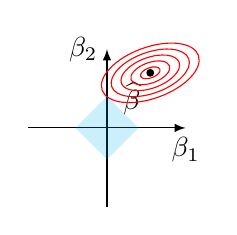
\begin{tikzpicture} 
                \draw[-latex] (-1,0) -- (1,0) node[below]{$\beta_1$};
                \draw[-latex] (0,-1) -- (0,1) node[left]{$\beta_2$};
                \fill[opacity=0.2,cyan] (-0.4,0) -- (0,-0.4) -- (0.4,0) -- (0,0.4) -- cycle;
                \coordinate[label=below left:$\widehat{\beta}$] (beta) at (0.55,0.7);
                \fill (beta) circle (0.5mm);
                \foreach \X in {0.13, 0.26, 0.39, 0.52, 0.65}
                {\draw[rotate=20,red] (beta) circle({1*\X} and {0.5*\X});}
            \end{tikzpicture}
            \end{center}
            \vspace{0.5cm}

            \( \sum_{j=1}^{p}\left|\beta_{j}\right| \) measures the models complexity. \( \lambda \) determines the penalty. \( \to \) we chose it with cross-validation.\\
            \textbf{Stepwise is a specific path through these models, but LASSO "searches" all combinations at once.}
        \end{multicols}
        Remember to refit!

\subsection{Trees}
Fit nonlinearities and selection automatically. We don't need to specify transformations ahead of time ( \( X^{2}_j \,\text{or} \, X_j \times X_k \) )
\begin{itemize}
    \item Initialize \(\hat{Y} = \overline{Y} \)
    \item For each \( X_j\)  one at a time, find cutoff \( t_j \) that most improves the predictions
        \[
            \hat{Y}=\left\{\begin{array}{ll}
                \bar{Y}_{X_{j} \leq t_{j}} & \text { if } X_{j} \leq t_{j} \\
                \bar{Y}_{X_{j}>t_{j}} & \text { if } X_{j}>t_{j}
                \end{array} \quad \bar{Y}_{X_{j} \leq t_{j}}=\frac{\sum_{i=1}^{n} Y_{i} \mathds{1}\left\{X_{j} \leq t_{j}\right\}}{\#\left\{X_{j} \leq t_{j}\right\}}\right.
        \] 
    \item Whatever single \( X_j, t_j \) is the best, keep that one Split
    \item Repeat, each time trying to improve one the prior iteration 
\end{itemize}

\begin{center}
\includegraphics[width=0.2\textwidth]{figures/trees.png}
\end{center}
\section{Time Series Analysis}

\begin{definition}{\textbf{Autoregressive Model}}
    \[
    AR(1): Y_{t} = \beta_0 + \beta_1 Y_{t-1} + \epsilon_{t}, \epsilon_{t} \sim N(0,\sigma^2)
    \] \\

    Previous lag values $\left(Y_{t-2}, Y_{t-3}, \ldots\right)$ do not help predict $Y_{t}$ if you already know $Y_{t-1}$.
\end{definition}

Correlation between \( Y_t \) and \( Y_{t-1} \) is called auto-correlation.
\vspace{0.2cm}

If $\left|\beta_{1}\right|>1$, the series explodes.
If $\left|\beta_{1}\right|=1$, we have a random walk.
If $\left|\beta_{1}\right|<1$, the values are mean reverting.
The random walk has some special properties ... $Y_{t}-Y_{t-1}=\beta_{0}+\varepsilon_{t}$, and $\beta_{0}$ is called the "drift parameter". The random walk without drift $\left(\beta_{0}=0\right)$ is a common model for simple processes
$-Y_{1}=\varepsilon_{1}, Y_{2}=\varepsilon_{1}+\varepsilon_{2}, Y_{3}=\varepsilon_{1}+\varepsilon_{2}+\varepsilon_{3}$, etc.
- the expectation of what will happen is always what happened most recently. $\mathbb{E}\left[Y_{t}\right]=Y_{t-1}$

\subsection{AR(p) Model}
$$
A R(p): Y_{t}=\beta_{0}+\beta_{1} Y_{t-1}+\cdots+\beta_{p} Y_{t-p}+\varepsilon
$$
\subsubsection{Trending Series}
Just put “time” in the model \(  Y_{t}=\beta_{0}+\beta_{1} Y_{t-1}+\beta_{2} t+\varepsilon_{t} \)
\subsubsection{Periodic Series}
Period $-k$ model :
$$
Y_{t}=\beta_{0}+\beta_{1} \sin (2 \pi t / k)+\beta_{2} \cos (2 \pi t / k)+\varepsilon_{t}
$$


\end{multicols}
\end{document}